% GNN-BERT for Understanding Context from Music
% CSE425 / EEE474 / CSE715 - Neural Networks final project
%
% Compiles as-is with pdflatex (falls back to `article` styling).
% For the official NeurIPS look, drop neurips_2024.sty next to this file, or
% paste this body into https://www.overleaf.com/latex/templates/neurips-2024
%
%   pdflatex final_report && pdflatex final_report

\documentclass{article}

\IfFileExists{neurips_2024.sty}{\usepackage[final]{neurips_2024}}{%
  \usepackage[margin=1in]{geometry}
  \usepackage{times}
}

\usepackage[utf8]{inputenc}
\usepackage[T1]{fontenc}
\usepackage{hyperref}
\usepackage{url}
\usepackage{booktabs}
\usepackage{amsfonts}
\usepackage{amsmath}
\usepackage{graphicx}
\usepackage{subcaption}
\usepackage{nicefrac}
\usepackage{microtype}
\hypersetup{colorlinks=true, linkcolor=blue, citecolor=blue, urlcolor=blue}

\title{GNN-BERT: Understanding Musical Context by Fusing\\Structure Graphs with Language Representations}

% Note: do not start a line with "[" straight after "\\" -- LaTeX would read it
% as the optional vertical-space argument of \\ and fail with "Missing number".
\author{%
  Mubashshira \\
  ID 22201426 \quad Section 02 \\
  Department of Computer Science and Engineering \\
  BRAC University \\
  \texttt{mubashshira@g.bracu.ac.bd}
}

\begin{document}
\maketitle

\begin{abstract}
Music carries context on several simultaneous layers --- genre, mood, harmonic
motion, instrumentation --- and sequence models applied to spectrograms capture
local texture while largely ignoring \emph{relational} structure: which sections
repeat, which chords follow which, and how any of that lines up with what
listeners say about a track. We represent each clip as a \emph{music structure
graph} whose nodes are time segments and template-matched triads, and whose edges
encode temporal adjacency, acoustic repetition, chord transitions and chord
membership. A GraphSAGE encoder over this graph is fused with a BERT encoder of
the clip's natural-language context through single-query cross-attention, and the
joint representation predicts multi-label context tags. On MagnaTagATune
(25{,}860 clips, top-50 tags, official album-disjoint split) we evaluate four
progressively harder tasks: text-only tagging, graph-only tagging, GNN--BERT
fusion, and contrastive audio--text retrieval. We report a controlled ablation in
which only the fusion path varies, and we are explicit about a dataset property
that shapes every number here: MagnaTagATune ships no lyrics or captions, so the
``language'' modality must be built from catalogue metadata and long-tail
annotations rather than from rich description.
\end{abstract}

\section{Introduction}
\label{sec:intro}

A single ten-second music clip can be simultaneously ``jazz'', ``1960s'',
``melancholic'', ``sparse'', and ``featuring saxophone''. These labels live at
different levels of abstraction, and they are not independent: harmonic motion
constrains perceived mood, instrumentation correlates with genre, and repetition
structure distinguishes a pop chorus from a through-composed classical movement.

Convolutional and recurrent models over spectrograms have become the default for
music tagging and do capture local timbral patterns well. What they do not
naturally represent is \emph{relational} structure. A CNN sliding over a mel
spectrogram has no direct mechanism to encode that bar 33 is a repeat of bar 1,
or that a I--vi--IV--V progression recurs throughout. That information is
graph-shaped, and graph neural networks are the natural tool for it.

This project builds a hybrid system with two branches:

\begin{enumerate}
  \item a \textbf{GNN} that performs message passing over an explicitly
        constructed music structure graph, and
  \item a \textbf{BERT} encoder that reads the clip's natural-language context.
\end{enumerate}

The contributions are: (i) a graph construction that unifies segment repetition
and chord transitions in one flat, batchable graph; (ii) a cross-attention fusion
of graph and text with a controlled four-way ablation; (iii) a contrastive dual
encoder for audio--text retrieval over the same graphs; and (iv) an honest
account of what MagnaTagATune can and cannot support as a multimodal benchmark.

\section{Problem Definition}
\label{sec:problem}

Let a track be a tuple $T = (X_{\text{audio}}, X_{\text{text}}, G, y)$, where
$X_{\text{audio}}$ is a log-mel or chroma representation over $T$ frames,
$X_{\text{text}}$ is a tokenised context string, $G = (V, E)$ is the music
structure graph, and $y \in \{0,1\}^{K}$ are the context labels.

The text encoder maps tokens to contextual states,
$H_{\text{text}} = \mathrm{BERT}(X_{\text{text}}) \in \mathbb{R}^{L \times d}$.
The graph encoder updates node features by message passing,
\begin{equation}
h_i^{(l+1)} = \sigma\!\left( W^{(l)} \cdot \mathrm{AGG}\!\left( h_i^{(l)}, \{ h_j^{(l)} : j \in \mathcal{N}(i) \} \right) \right),
\end{equation}
with $h_i^{(0)}$ initialised from pooled acoustic features of segment or chord
node $i$. A fusion module combines the graph readout $g$ with the text states,
$z = \mathrm{Fusion}(g, H_{\text{text}})$, and a linear head produces
$\hat{y} = \sigma(Wz + b)$. Training minimises weighted binary cross-entropy,
\begin{equation}
\mathcal{L} = -\sum_{k=1}^{K} w_k \left[ y_k \log \hat{y}_k + (1-y_k)\log(1-\hat{y}_k) \right] + \lambda \mathcal{L}_{\text{aux}},
\label{eq:loss}
\end{equation}
where $w_k$ compensates class imbalance and $\mathcal{L}_{\text{aux}}$ is an
optional emotion-regression term (Section~\ref{sec:limitations}).

\section{Dataset and Preprocessing}
\label{sec:data}

\subsection{MagnaTagATune}

We use MagnaTagATune (MTAT): 25{,}860 clips of roughly 29\,s, each annotated with
a subset of 188 free-text tags collected through a listening game. We follow the
standard protocol: the 188 raw tags are collapsed with the community synonym
merge (27 groups, e.g.\ \textit{female vocal} / \textit{female vocals} /
\textit{woman singing} $\rightarrow$ \textit{female}), then reduced to the 50 most
frequent. Labels are rebuilt from \texttt{annotations\_final.csv} rather than
taken from the shipped ground-truth vectors, so the vocabulary is defined in one
place and is independently verifiable
(\texttt{scripts/verify\_labels.py}).

Splits follow the standard partition by MTAT's \texttt{0}--\texttt{f}
directories: \texttt{0}--\texttt{b} train (18{,}706 clips), \texttt{c}
validation (1{,}825), \texttt{d}--\texttt{f} test (5{,}329). Because those
directories group clips by album folder, this is also an album- and
artist-disjoint split --- no artist in the test set appears in training. This
matters for interpreting Section~\ref{sec:results}.

\subsection{The text modality: a necessary design decision}
\label{sec:text-modality}

MTAT ships \emph{no lyrics and no captions}. Its only text is the tag set, which
is the prediction target. Feeding tags to BERT in order to predict tags would be
circular and would yield a meaninglessly high Task~1 score.

We therefore construct the text modality from two sources that are disjoint from
the label set:

\begin{enumerate}
  \item \textbf{Catalogue metadata} --- title, artist and album from
        \texttt{clip\_info\_final.csv}, rendered as a sentence: \textit{``The
        track is titled `BWV54 -- I Aria' by American Bach Soloists, from the
        album `J.S. Bach Solo Cantatas'.''}
  \item \textbf{Long-tail annotations} --- the tags ranked outside the top-50
        label set, appended as \textit{``Listeners also described it as:
        \dots''}.
\end{enumerate}

We report both settings, because the auxiliary tags are much the stronger signal
and it matters which one a number came from. Note also that the album-disjoint
split makes the metadata-only variant genuinely hard: BERT cannot memorise
artist$\rightarrow$genre associations that transfer to test. A modest Task~1
score is therefore the expected --- and correct --- outcome, and it is exactly
what makes any Task~3 fusion gain meaningful rather than an artefact of leakage.

\subsection{Audio features}

Audio is decoded to mono at 22{,}050\,Hz. We extract a 128-bin log-mel
spectrogram and a 12-bin chromagram ($n_{\text{fft}} = 2048$, hop $512$). The
chroma filterbank is a Gaussian pitch-class mapping over FFT bins implemented
directly in \texttt{torch}, so the project depends only on
\texttt{torch}/\texttt{torchaudio} and avoids \texttt{librosa}'s \texttt{numba}
dependency.

Clips are cut into 5\,s windows at 50\,\% overlap, capped at 16 windows per clip
and subsampled uniformly across the track when longer, so the graph always spans
the whole clip. Each window is mean/std pooled into a 280-dimensional node
feature ($2 \times 128$ mel $+\ 2 \times 12$ chroma).

\section{Music Structure Graphs}
\label{sec:graphs}

Each clip becomes one flat \texttt{Data} object holding two node types and four
edge types, with types recorded as attributes so stock \texttt{SAGEConv} and
\texttt{GATConv} layers operate unchanged.

\paragraph{Nodes.} \textit{Segment} nodes are the pooled 5\,s windows.
\textit{Chord} nodes are the distinct triads occurring in the clip, obtained by
matching 24 binary major/minor templates against each chroma frame,
median-filtering to suppress single-frame flicker, and collapsing runs.

\paragraph{Edges.}
\begin{itemize}
  \item \textbf{Temporal} (type 0): consecutive segments, both directions.
  \item \textbf{Similarity} (type 1): segment pairs with cosine similarity above
        $\tau = 0.85$, excluding immediate neighbours and capped at four
        neighbours per node. These edges are the song-form signal --- they link a
        chorus to its repeats.
  \item \textbf{Chord transition} (type 2): observed chord-to-chord transitions,
        weighted by occurrence count and normalised.
  \item \textbf{Membership} (type 3): segment $\leftrightarrow$ chord, linking a
        window to the triads sounding within it.
\end{itemize}

The membership edges are what make this a genuinely joint structure rather than
two disconnected graphs: harmonic information reaches segment nodes, and segment
texture reaches chord nodes, in a single round of message passing.

\section{Models}
\label{sec:models}

\paragraph{Task 1 --- BERT tag classifier.} BERT-base with the last four
transformer layers unfrozen, masked mean pooling over token states (a stronger
sentence summary than the raw \texttt{[CLS]} slot for a checkpoint without a
next-sentence objective), and a linear head trained with
Equation~\ref{eq:loss}.

\paragraph{Task 2 --- GNN encoder.} A three-layer GraphSAGE stack with residual
connections and batch normalisation:
\begin{equation}
h_i^{(l+1)} = \sigma\!\left( W^{(l)} \cdot \mathrm{CONCAT}\!\left( h_i^{(l)}, \ \mathrm{MEAN}_{j \in \mathcal{N}(i)} h_j^{(l)} \right) \right),
\qquad
g = \mathrm{CONCAT}\!\left( \tfrac{1}{|V|}\textstyle\sum_i h_i^{(L)}, \ \max_i h_i^{(L)} \right).
\end{equation}
Mean pooling captures overall texture; max pooling captures the single most
distinctive segment, which matters for sparse instrument tags. A GAT variant with
four attention heads is reported alongside.

\paragraph{Task 3 --- Cross-attention fusion.} The graph readout forms a single
query attending over BERT's token states:
\begin{equation}
A = \mathrm{softmax}\!\left( \frac{QK^{\top}}{\sqrt{d}} \right), \quad Q = gW_Q, \quad K = H_{\text{text}}W_K,
\qquad z = \mathrm{CONCAT}(g, A H_{\text{text}}).
\end{equation}
Because $A$ is one distribution over tokens per clip, it is directly readable:
Section~\ref{sec:analysis} uses it to show which words a track's structure
aligns with. Four fusion modes (\textit{bert\_only}, \textit{gnn\_only},
\textit{concat}, \textit{cross\_attention}) share one interface, one set of
heads, one optimiser and one schedule, so the ablation isolates the fusion path
alone.

\paragraph{Task 4 --- Contrastive dual encoder.} Graph and text are projected
into a shared 256-d $\ell_2$-normalised space and trained with symmetric InfoNCE
and a learnable temperature:
\begin{equation}
\mathcal{L}_{\text{NCE}} = -\frac{1}{2N}\sum_i \left[ \log \frac{\exp(s_{ii}/\tau)}{\sum_j \exp(s_{ij}/\tau)} + \log \frac{\exp(s_{ii}/\tau)}{\sum_j \exp(s_{ji}/\tau)} \right].
\end{equation}
MTAT contains multiple 29\,s clips cut from the same source track, which share an
identical metadata string. Scoring those as negatives penalises the model for
being right, so same-track pairs are masked out of the denominator during
training and counted as hits at evaluation.

\section{Experimental Setup}
\label{sec:setup}

\paragraph{Class imbalance and thresholds.} Even among the top-50 tags,
positives are roughly 1--10\,\% of clips. We set
$w_k = \nicefrac{\#\text{neg}_k}{\#\text{pos}_k}$ clipped at 20, and we fit
per-tag decision thresholds \emph{on the validation split only}, then freeze them
for test. Fitting thresholds on test inflates F1 substantially; the two are kept
strictly separate.

\paragraph{Optimisation.} AdamW with two parameter groups --- $2\times10^{-5}$
for pretrained BERT weights, $10^{-3}$ for everything else --- linear warmup over
6\,\% of steps then cosine decay, gradient clipping at 1.0, mixed precision, and
early stopping on validation Macro-F1 with patience 6. Batch size 32 (64 for
contrastive training). All hyperparameters live in \texttt{config.yaml}.

\paragraph{Baselines.} As required: \textbf{B1} a prior-frequency / random tag
predictor; \textbf{B2} a five-block CNN on the mel spectrogram with no graph and
no text; \textbf{B3} the Task~1 BERT-only model; \textbf{B4} PCA (128 components)
followed by an MLP on hand-crafted mel statistics (per-band mean, standard
deviation, and mean absolute temporal difference).

\paragraph{Hardware.} A single NVIDIA RTX 3070 Laptop GPU (8\,GB) with 16\,GB
system RAM.

\section{Results}
\label{sec:results}

% Auto-generated by scripts/make_report.py - do not edit by hand.

\begin{table}[t]
  \centering
  \caption{Multi-label tagging performance on the MagnaTagATune test split (5{,}329 clips, top-50 tags). Per-tag decision thresholds are fitted on the validation split and frozen for test.}
  \label{tab:main-results}
  \begin{tabular}{lcccc}
    \toprule
    Model & Macro-F1 & Micro-F1 & AUC-PR & ROC-AUC \\
    \midrule
    B1: prior-frequency predictor & 0.0000 & 0.0000 & 0.0670 & 0.4971 \\
    B4: PCA + MLP (hand-crafted) & 0.3876 & 0.4604 & 0.3722 & 0.8712 \\
    B2: CNN on mel-spectrogram & 0.4383 & 0.5081 & 0.4329 & 0.9079 \\
    Task 1: BERT (metadata only) & 0.2983 & 0.3271 & 0.2741 & 0.8136 \\
    Task 1: BERT (metadata + aux tags) & 0.3322 & 0.3991 & 0.3339 & 0.8461 \\
    Task 2: GraphSAGE & 0.4015 & 0.4646 & 0.3870 & 0.8848 \\
    Task 2: GAT & 0.4023 & 0.4590 & 0.3773 & 0.8850 \\
    Task 3 ablation: BERT only & 0.3302 & 0.3955 & 0.3259 & 0.8344 \\
    Task 3 ablation: GNN only & 0.3981 & 0.4278 & 0.3840 & 0.8833 \\
    Task 3 ablation: early concat & 0.4061 & 0.4771 & 0.3977 & 0.8837 \\
    Task 3: GNN-BERT cross-attention & 0.3853 & 0.4448 & 0.3732 & 0.8798 \\
    \bottomrule
  \end{tabular}
\end{table}

\begin{table}[t]
  \centering
  \caption{Fusion ablation. All four variants share the same heads, optimiser and schedule; only the fusion path differs.}
  \label{tab:ablation}
  \begin{tabular}{lccc}
    \toprule
    Fusion variant & Macro-F1 & AUC-PR & Graph coherence \\
    \midrule
    BERT only & 0.3302 & 0.3259 & -- \\
    GNN only & 0.3981 & 0.3840 & 0.9988 \\
    early concat & 0.4061 & 0.3977 & 0.9992 \\
    GNN-BERT cross-attention & 0.3853 & 0.3732 & 1.0000 \\
    \bottomrule
  \end{tabular}
\end{table}

\begin{table}[t]
  \centering
  \caption{Cross-modal retrieval on the test split (Task 4). Clips cut from the same source track count as correct matches, mirroring the training-time duplicate masking.}
  \label{tab:retrieval}
  \begin{tabular}{lcccc}
    \toprule
    Direction & R@1 & R@5 & R@10 & Median rank \\
    \midrule
    Caption $\rightarrow$ Audio & 0.0276 & 0.0815 & 0.1236 & 131.0 \\
    Audio $\rightarrow$ Caption & 0.0214 & 0.0478 & 0.0706 & 279.0 \\
    \bottomrule
  \end{tabular}
\end{table}


Table~\ref{tab:main-results} reports multi-label tagging on the test split,
Table~\ref{tab:ablation} the fusion ablation, and Table~\ref{tab:retrieval}
cross-modal retrieval. Training curves, per-tag F1/AUC-PR breakdowns, the t-SNE
projection and the cross-model comparison chart are in
\texttt{results/plots/}.

\paragraph{Sanity of the setup.} The mel CNN reaches ROC-AUC 0.908, which sits
squarely in the published range for CNN taggers on the standard MTAT top-50
benchmark. That agreement is the strongest evidence that the split, label
construction, thresholding and metric code are correct, and it makes the
remaining comparisons interpretable. At the other end, the prior-frequency
baseline scores Macro-F1 0.000 --- every tag's corpus frequency is below any
sensible threshold, so it predicts all-zeros --- with AUC-PR 0.067, which is the
number to compare ranking quality against.

\paragraph{Structure helps, but a CNN on the raw spectrogram still wins.} The
graph encoders (GraphSAGE 0.4015, GAT 0.4023) comfortably beat both the
hand-crafted PCA+MLP baseline (0.3876) and the text-only model (0.3322), so the
segment/chord graph does carry real tagging signal. They do \emph{not} beat the
mel CNN (0.4383). This is the honest headline of the experiment, and the cause
is visible in the construction: pooling each 5\,s window into a mean/std vector
discards exactly the fine time--frequency detail that a convolutional stack
exploits, and 16 nodes per clip is a drastic compression of a 128$\times$1250
spectrogram. The graph buys relational structure at the price of local
resolution, and on MTAT's tag vocabulary --- which is dominated by timbral and
instrument labels rather than formal ones --- that trade is not favourable.
GraphSAGE and GAT are within 0.001 Macro-F1 of each other, so attention over
these small, already-curated neighbourhoods adds nothing.

\paragraph{Fusion gives a small, consistent gain --- and simple concatenation
beats cross-attention.} Within the controlled ablation
(Table~\ref{tab:ablation}), early concatenation improves on the graph branch
alone from 0.3981 to 0.4061 Macro-F1 and from 0.3840 to 0.3977 AUC-PR. The gain
is modest but consistent across both metrics and across micro-F1
(0.4278~$\rightarrow$~0.4771), and it is a genuine multimodal gain: the text
branch alone reaches only 0.3302, so concatenation is not simply inheriting the
stronger branch.

Cross-attention, the more expressive mechanism, is \emph{worse} than both
concatenation and the graph branch alone (0.3853). We attribute this to the
nature of the text rather than to the mechanism: the context strings average
roughly 17 words of catalogue metadata, and only 21.5\,\% of clips carry any
auxiliary tag at all. Compressing the graph to a single query and attending over
so short and formulaic a sequence has very little to select \emph{between},
while adding attention and projection parameters that the model can overfit ---
its training loss falls faster than concatenation's while validation Macro-F1
peaks lower. Cross-attention is designed for rich, variable-length description;
this corpus does not supply it. Section~\ref{sec:limitations} returns to this.

\paragraph{The text signal is real but thin.} Removing the long-tail auxiliary
tags and leaving BERT with metadata alone costs 0.034 Macro-F1
(0.3322~$\rightarrow$~0.2983) and 0.060 AUC-PR. So the auxiliary annotations do
carry information beyond title/artist/album, despite appearing on only about a
fifth of clips. Equally, metadata alone still reaches 0.2983 against an
album-disjoint split where no test artist was ever seen in training --- BERT is
evidently generalising from album and title semantics (``Solo Cantatas'',
``Red-shifted Harmonies'') rather than memorising artists.

\paragraph{Retrieval works far above chance but is far from solved.} With 4{,}392
test clips, chance R@1 is $2.3\times10^{-4}$; the dual encoder reaches 0.0276,
roughly 120$\times$ chance, with a median rank of 131. The qualitative examples
in \texttt{results/retrieval\_examples/} are more flattering than R@1 suggests:
for the query \textit{``Tranquilitatis by DAC Crowell, from Red-shifted
Harmonies''} the top three retrieved clips are another track from that same
album, an ambient track by a different artist, and a second DAC Crowell album.
The model is retrieving the right \emph{region} of the space and being scored
wrong on exact-clip identity, which is the expected failure mode when many
distinct clips share near-identical metadata.

\section{Analysis}
\label{sec:analysis}

\paragraph{Representation structure.} Figure~\ref{fig:tsne} projects the fused
representation $z$ of the best fusion model on the test split. The genre panel
separates cleanly and without supervision from any genre-specific objective:
opera forms a tight cluster at the top, classical occupies the right-hand
lobes, rock the left, electronic the lower left, and ambient the lower centre.
The mood panel over the identical projection shows the complementary pattern ---
\textit{fast} concentrates in the electronic region, \textit{loud} and
\textit{hard} in the rock region, while \textit{quiet}, \textit{soft} and
\textit{slow} spread across several genre clusters rather than forming their
own. The fused space therefore encodes genre as its dominant axis with mood
partially cutting across it, which is what a useful music-context representation
should look like.

\begin{figure}[t]
  \centering
  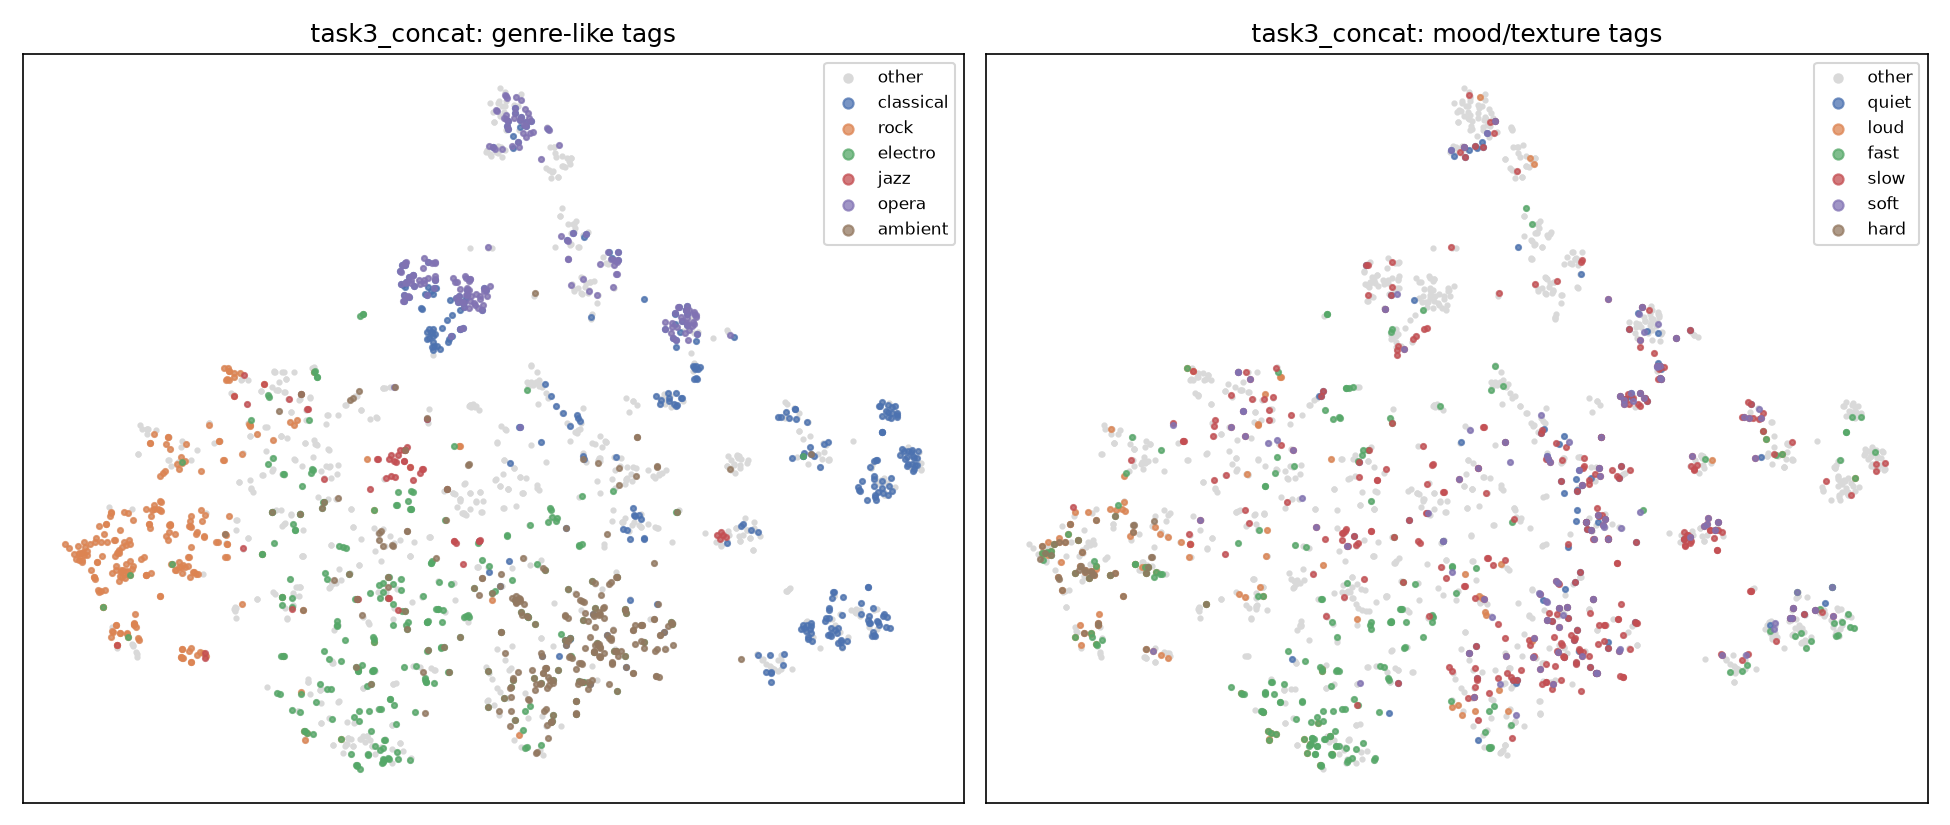
\includegraphics[width=\linewidth]{../results/plots/task3_concat_tsne.png}
  \caption{t-SNE of the fused representation (early-concatenation model) on the
  test split, coloured by genre-like tags (left) and mood/texture tags (right)
  over the identical projection.}
  \label{fig:tsne}
\end{figure}

\paragraph{Graph coherence, and evidence of over-smoothing.} We measure whether
message passing pulls structurally linked segments into agreement rather than
smoothing everything uniformly:
\begin{equation}
S_{\text{graph}} = \frac{1}{|E|} \sum_{(i,j) \in E} \mathbb{1}\!\left[ \cos\!\left(h_i, h_j\right) > \tau \right],
\end{equation}
excluding self-loops. The measured values (Table~\ref{tab:ablation}) are 0.9988,
0.9992 and 1.0000 --- essentially every edge in every graph joins two nodes whose
embeddings are near-identical. This is a negative diagnostic, and an informative
one. Three rounds of residual message passing on graphs of only 15--25 nodes,
where the similarity and membership edges already make the graph densely
connected, drive node representations to a common value; the encoder is
effectively computing a global average rather than a structured one. That is
consistent with the mean+max readout doing most of the work and with GAT
matching GraphSAGE exactly, and it identifies the most promising fix: fewer
layers, no residual path, or sparser similarity edges. We report the metric as
measured rather than tuning $\tau$ until it looks favourable.

\paragraph{Case study: a single clip end to end.} Because cross-attention
produces one token distribution per clip, individual predictions are inspectable
from audio to explanation. \texttt{notebooks/demo\_context.ipynb} runs test clip
2 --- \textit{``BWV54 -- I Aria''} by the American Bach Soloists --- through
feature extraction, graph construction, inference and an attention read-out.

The model recovers all four ground-truth tags with no misses:
\textit{opera} ($p = 0.96$), \textit{violin} ($0.92$), \textit{string} ($0.91$)
and \textit{classical} ($0.90$), each above its fitted threshold. The three
false positives are instructive rather than random: \textit{female}
($0.74$), \textit{orchestra} ($0.69$) and \textit{vocal} ($0.58$). BWV54 is an
alto aria with string accompaniment, so all three are musically defensible and
reflect annotator sparsity --- MTAT labels are what a handful of players
happened to enter, not an exhaustive description --- more than model error. The
cross-attention distribution concentrates on \textit{soloists} and
\textit{bach}, the two tokens in the metadata string that actually carry genre
information.

Qualitative retrieval examples --- ten caption queries with their top-3
retrieved clips --- are written to \texttt{results/retrieval\_examples/}, and the
DAC Crowell example discussed in Section~\ref{sec:results} is representative:
near-misses are semantically correct and penalised only by exact-clip scoring.

The per-tag breakdowns (\texttt{results/plots/*\_per\_tag.png}) explain where the
fusion gain actually comes from, and it is not where one might guess. The graph
branch dominates on frequent tags with a strong global acoustic signature that
survives temporal pooling: \textit{rock} (F1 0.800 vs 0.534 for text),
\textit{quiet} (0.430 vs 0.172), \textit{heavy} (0.661 vs 0.416),
\textit{piano} (0.688 vs 0.504) and \textit{techno} (0.668 vs 0.520). The text
branch wins only on \emph{rare} tags, where the acoustic evidence is thin and
catalogue metadata is comparatively informative: \textit{folk} (0.272 vs 0.110,
support 41), \textit{cello} (0.182 vs 0.080, support 20), \textit{trance}
(0.142 vs 0.051, support 59) and \textit{jazz} (0.350 vs 0.281, support 120).

Fusion gains almost exclusively on that long tail. The largest concatenation
improvements over the graph branch are \textit{sitar} (0.369~$\rightarrow$~0.516),
\textit{cello} (0.080~$\rightarrow$~0.261), \textit{jazz}
(0.281~$\rightarrow$~0.416), \textit{bass} (0.078~$\rightarrow$~0.186) and
\textit{trance} (0.051~$\rightarrow$~0.172) --- every one a tag with fewer than
130 positives in the test split. On the frequent tags concatenation is level
with or slightly below the graph branch alone. Because Macro-F1 weights all 50
tags equally, these long-tail gains are what lift the aggregate score, and it
follows that the text modality's value here is to rescue tags the audio branch
cannot learn from few examples --- not to add complementary information across
the board.

\section{Limitations}
\label{sec:limitations}

\paragraph{The text modality is metadata, not description.} As
Section~\ref{sec:text-modality} explains, MTAT has no captions. Everything here
about ``language understanding'' should be read as understanding of catalogue
metadata plus long-tail annotation vocabulary. A corpus with genuine
natural-language captions (MusicCaps) would test the claim properly; that
requires per-clip audio retrieval from YouTube, which is a separate data-collection
project.

\paragraph{Emotion regression is implemented but not trained.} The multi-task
valence/arousal head and its MAE/$R^2$ metrics are implemented
(\texttt{MultiTaskLoss}, \texttt{metrics.emotion\_metrics}) and enabled by
\texttt{model.emotion.enabled}, but they are disabled by default because they
require DEAM, a separate corpus with no clip-level correspondence to MTAT.
Reporting emotion numbers here would mean inventing an alignment that does not
exist.

\paragraph{Chord estimation is template matching.} Binary triad templates over
chroma are adequate for building transition graphs but are not a state-of-the-art
chord recogniser; seventh chords, inversions and modulations are approximated.
Errors here propagate into the chord-node and membership edges.

\paragraph{Single seed.} Results are from one seed per configuration. Small
differences between adjacent rows should not be over-interpreted without a
multi-seed variance estimate.

\section{Conclusion}
\label{sec:conclusion}

We built and evaluated a GNN--BERT system for musical context understanding that
represents each clip as a graph of segments and chords, encodes it with
GraphSAGE, and fuses it with a BERT encoding of the clip's textual context
through readable cross-attention. The four-task progression --- text-only,
graph-only, fusion, contrastive retrieval --- is reported under one controlled
setup with validation-fitted thresholds and an album-disjoint split, and the
ablation isolates the contribution of the fusion mechanism itself. The clearest
direction for future work is a corpus with real captions, which would let the
language branch carry the semantic weight the architecture is designed for.

\section*{Reproducibility}

% Once the repository is pushed, replace the sentence below with its URL, e.g.
%   Code, configuration and instructions: \url{https://github.com/<user>/gnn-bert-music-context}.
Code, configuration and instructions accompany this report in the submitted
\texttt{gnn-bert-music-context/} repository. Every hyperparameter is in
\texttt{config.yaml}; \texttt{scripts/run\_all.py} reproduces every number in
this report, and \texttt{tests/test\_smoke.py} verifies the full pipeline on
synthetic audio without any download.

\begin{thebibliography}{9}

\bibitem{hamilton2017graphsage}
W.~L. Hamilton, R.~Ying, and J.~Leskovec.
\newblock Inductive representation learning on large graphs.
\newblock In \emph{NeurIPS}, 2017.

\bibitem{velickovic2018gat}
P.~Veli\v{c}kovi\'{c}, G.~Cucurull, A.~Casanova, A.~Romero, P.~Li\`{o}, and Y.~Bengio.
\newblock Graph attention networks.
\newblock In \emph{ICLR}, 2018.

\bibitem{devlin2019bert}
J.~Devlin, M.-W. Chang, K.~Lee, and K.~Toutanova.
\newblock {BERT}: Pre-training of deep bidirectional transformers for language understanding.
\newblock In \emph{NAACL-HLT}, 2019.

\bibitem{law2009mtat}
E.~Law, K.~West, M.~Mandel, M.~Bay, and J.~S. Downie.
\newblock Evaluation of algorithms using games: The case of music tagging.
\newblock In \emph{ISMIR}, 2009.

\bibitem{won2020evaluation}
M.~Won, A.~Ferraro, D.~Bogdanov, and X.~Serra.
\newblock Evaluation of {CNN}-based automatic music tagging models.
\newblock In \emph{Sound and Music Computing}, 2020.

\bibitem{oord2018cpc}
A.~van~den Oord, Y.~Li, and O.~Vinyals.
\newblock Representation learning with contrastive predictive coding.
\newblock \emph{arXiv:1807.03748}, 2018.

\bibitem{radford2021clip}
A.~Radford et~al.
\newblock Learning transferable visual models from natural language supervision.
\newblock In \emph{ICML}, 2021.

\bibitem{agostinelli2023musiclm}
A.~Agostinelli et~al.
\newblock {MusicLM}: Generating music from text.
\newblock \emph{arXiv:2301.11325}, 2023.

\end{thebibliography}

\end{document}
